\documentclass[aspectratio=169,11pt]{beamer}

% Shared style (ib-tutorials.sty at the repo root).
\makeatletter\def\input@path{{./}{../}}\makeatother
\usepackage{ib-tutorials}

\usepackage[utf8]{inputenc}
\usepackage{amsmath,amssymb}
\usepackage{booktabs}
\usepackage{array}
\newcolumntype{L}[1]{>{\raggedright\arraybackslash}p{#1}}
\usepackage{graphicx}
\graphicspath{{../pictures/3-ibamr-fundamentals/}{pictures/3-ibamr-fundamentals/}}
\usepackage{xcolor}
\usepackage{listings}
\usepackage{tikz}
\usetikzlibrary{arrows.meta,positioning,shapes.geometric,fit,calc}
\usepackage{hyperref}

\newcommand{\sourcecredit}[1]{\vfill\begin{flushright}\tiny\textcolor{DarkGray}{#1}\end{flushright}}

\lstset{
  basicstyle=\ttfamily\scriptsize\color{BlackGray},
  keywordstyle=\color{NavyBlue}\bfseries,
  commentstyle=\color{DarkGray}\itshape,
  stringstyle=\color{OliveGreen},
  showstringspaces=false,
  columns=fullflexible,
  keepspaces=true,
  breaklines=true,
  breakindent=1em,
  frame=single,
  framerule=0.4pt,
  rulecolor=\color{LightGray},
  backgroundcolor=\color{LightGray!30},
  xleftmargin=0.25em,
  xrightmargin=0.25em
}
\lstdefinestyle{shell}{morecomment=[l]{\#}}
\lstdefinestyle{input}{morecomment=[l]{//}}
\lstdefinestyle{matlab}{morecomment=[l]{\%}}
\lstdefinestyle{python}{morecomment=[l]{\#}}
\lstdefinestyle{data}{}
\lstdefinestyle{tiny}{basicstyle=\ttfamily\tiny\color{BlackGray}}
\lstdefinestyle{inputtiny}{morecomment=[l]{//},basicstyle=\ttfamily\tiny\color{BlackGray}}
\lstdefinestyle{matlabtiny}{morecomment=[l]{\%},basicstyle=\ttfamily\tiny\color{BlackGray}}
\lstdefinestyle{pythontiny}{morecomment=[l]{\#},basicstyle=\ttfamily\tiny\color{BlackGray}}
\lstdefinestyle{cpp}{language=C++,morecomment=[l]{//}}
\lstdefinestyle{cpptiny}{language=C++,morecomment=[l]{//},basicstyle=\ttfamily\tiny\color{BlackGray}}
\lstdefinestyle{cmake}{morecomment=[l]{\#}}

\title[Output and analysis of forces]{Output and analysis of forces}
\subtitle{What IBAMR's forces are, how the examples write them and the positions to disk, and how to read, sum, normalize and filter them in Python and MATLAB}
\author[Miller]{Laura A. Miller}
\institute[UArizona]{Department of Mathematics, University of Arizona}
\date{Using IB Software \textbullet\ Part III \textbullet\ Chapter 11}

\begin{document}

% 1
\begin{frame}[plain]
\maketutorialtitlepanel{%
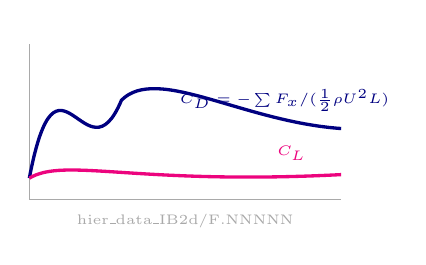
\begin{tikzpicture}[scale=0.9]
  \draw[DarkGray] (0,0) -- (4.4,0); \draw[DarkGray] (0,0) -- (0,2.2);
  \draw[NavyBlue,very thick] (0,0.3) .. controls (0.4,2.4) and (0.8,0.2) .. (1.3,1.4) .. controls (1.8,1.9) and (3.0,1.1) .. (4.4,1.0);
  \draw[RubineRed,very thick] (0,0.3) .. controls (0.5,0.6) and (1.5,0.2) .. (4.4,0.35);
  \node[font=\tiny,text=NavyBlue] at (3.6,1.4) {$C_D = -\sum F_x / (\tfrac12\rho U^2 L)$};
  \node[font=\tiny,text=RubineRed] at (3.7,0.65) {$C_L$};
  \node[font=\tiny,text=DarkGray] at (2.2,-0.3) {\code{hier\_data\_IB2d/F.NNNNN}};
\end{tikzpicture}}
\end{frame}

% 2
\begin{frame}{Learning goals}
\label{fr:goals}
\footnotesize By the end of this chapter you should be able to:
\begin{enumerate}
  \item say what the numbers in IBAMR's Lagrangian force are (forces, not force densities; the force the structure exerts on the fluid) and what the sum over a structure means (the tether and applied forces; minus the force of the fluid on the body);
  \item find and read the \code{X.NNNNN} and \code{F.NNNNN} files that the examples write (format, ordering, time stamps), in Python and in MATLAB, with the readers shipped in \code{examples/analysis};
  \item turn the summed force into a drag or lift coefficient, with the course's $\frac12\rho U^2 S$ and chapter 8b's $\rho U^2 L$, and know where the factor 2 and the minus sign come from;
  \item measure kinematics from the positions (a tip, a marker cloud, a structure's extent), as every figure of chapters 7--10 did, and filter a noisy force signal without hiding the physics;
  \item know the other outputs IBAMR offers (the Silo Lagrangian data for VisIt, the upstream examples' own drag and lift, callbacks) and where chapter 33 takes the Eulerian fields into MATLAB.
\end{enumerate}
\begin{punchbox}
\footnotesize The forces are the quantity a biologist or an engineer wants from an IB simulation: thrust, drag, lift, work. Everything in this chapter is a few lines of reading and summing; the care goes into signs, factors and ordering.
\end{punchbox}
\end{frame}

% 3
\begin{frame}{How this chapter was checked}
\label{fr:checked}
\begin{itemize}\footnotesize
  \item The file format is taken from files written by the examples with IBAMR 0.19.0 on 1 and 3 processes (slide \ref{fr:format}), and the writer is the examples' own \code{output\_data()}, quoted in full; the course's slides and scripts assumed a layout (``three header lines'') that holds for the files they had and is checked here against the current ones.
  \item The readers (\code{hier\_data.py}, \code{read\_hier\_data.m}) and the analysis of the tethered leaf (\code{leaf\_forces.py}, \code{leaf\_forces.m}) were run on IB/03's output with Python 3.12 and Octave 8.4; the table and figure are theirs, and the numbers agree between the two.
  \item The 2013 claim ``there is a scaling error in IBAMR, so all forces need to be divided by 2'' is examined on slide \ref{fr:coeffs}: the factor is the $\frac12$ of the dynamic pressure in the coefficient's definition, and the course's own script applied it as such; no later edition repeated the claim.
  \item The course's \code{Example\_FruitFly\_Re10} (\code{Example\_output\_forces.zip}) is no longer in the folders; its figure and its script (\code{dataread2.m}, from the public \code{Reading-Forces} folder) are described and quoted, and the method is demonstrated on IB/03 instead.
\end{itemize}
\begin{punchbox}
\footnotesize Slide numbers refer to this deck; chapter numbers (6, 7, 8b, 9a, 9b, 10, 16, 26, 33, 36) to the other chapters of this series.
\end{punchbox}
\end{frame}

% 4
\begin{frame}{Where to look things up}
\label{fr:lookup}
\small
\begin{itemize}
  \item \al{The writer}: \code{output\_data()} at the end of every example's \code{main.cpp} of this series (slide \ref{fr:writer}); it comes from IBAMR's \code{examples/IB/explicit/ex1}, which also shows how to write the Eulerian fields to HDF5.
  \item \al{The readers}: \code{examples/analysis/hier\_data.py} (Python: \code{read\_vec}, \code{read\_series}, \code{read\_input}) and \code{read\_hier\_data.m}, \code{read\_input.m} (MATLAB/Octave), with \code{leaf\_forces.py} and \code{leaf\_forces.m} as worked examples; the course's \code{dataread2.m} and the lab's 3D script are quoted on slides \ref{fr:dataread} and \ref{fr:threed}.
  \item \al{The input keys}: \code{data\_dump\_interval} and \code{data\_dump\_dirname} in the \code{Main} block of every input file; \code{viz\_dump\_interval} next to them (chapter 7's input tour).
  \item \al{What the force is}: the IBAMR FAQ, \url{https://github.com/IBAMR/IBAMR/wiki/FAQ} (``forces, not force densities''); chapter 6 (the $\Delta s$ in every stiffness), chapter 8b (the dimensionless forces).
  \item \al{Eulerian data into MATLAB}: chapter 33 (the \code{importsamrai} tools of the 2013 lecture, VisIt's export); chapter 26 for VisIt itself.
  \item The class documentation, \url{https://ibamr.github.io/docs}: \code{LDataManager}, \code{LData}, \code{LSiloDataWriter}.
\end{itemize}
\end{frame}

% 5
\begin{frame}{Forces, not force densities}
\label{fr:faq}
\small From the IBAMR FAQ, quoted in every edition of this lecture (2012, 2013, 2015, 2017, 2020):
\begin{quote}\footnotesize
``Although force densities are more natural in the continuum setting, the Lagrangian data structures implemented in IBAMR are not sophisticated enough to use force densities. To simplify the software interface, we decided to make all Lagrangian forces actual forces (not force densities). Note that this convention affects the units required for spring constants, bending stiffnesses, etc.

Essentially, if you have a Lagrangian elasticity model that is phrased in terms of force densities, you must convert it into a model that is phrased in terms of forces in order to use this model with IBAMR. If $\mathbf{F}$ is the force passed to IBAMR and $\tilde{\mathbf{F}}$ is the original force density, what you need to compute is something like $\mathbf{F}(s,t) = \tilde{\mathbf{F}}(s,t)\,dV$, where $dV$ is the appropriate (discrete) volume element.''
\end{quote}
\vspace{1mm}
\footnotesize ``The new force version of IBAMR will output the forces applied to the fluid. Note these are also forces (not force densities).'' (2012) Every IBAMR since has had this; ``the new force version'' was the 2012 build at UNC.
\end{frame}

% 6
\begin{frame}{What that means for your model and your files}
\label{fr:units}
\small
\begin{itemize}
  \item Every number in \code{F.NNNNN} is a \al{force on one point} (N in SI; per unit depth in 2D, so N/m), not a force per unit length or area. Summing the numbers of a structure gives a force; integrating is not needed, since $dV$ is already inside.
  \item The $\Delta s$ factors of chapter 6 are exactly the ``$\tilde{\mathbf{F}}\,dV$'' conversion: a spring stiffness $K$ per unit strain becomes $K/\Delta s$ in the file, a bending stiffness $k_b$ becomes $k_b/\Delta s^3$, a tether stiffness $\kappa$ becomes $\kappa/\Delta s$ (IB/03's generator comments say which). Get the factor wrong and the file's forces are wrong by that factor, with no warning.
  \item The force in the file is the force \al{the structure exerts on the fluid}: it is what IBAMR spreads onto the grid. The force the fluid exerts on the structure is its negative (slide \ref{fr:sum}).
  \item Chapter 8b's dimensionless force, $F' = F/(\rho U^2 L)$ in 2D or $F/(\rho U^2 L^2)$ in 3D, divides this summed force; the course's coefficient (slide \ref{fr:coeffs}) differs by the $\frac12$.
\end{itemize}
\begin{punchbox}
\footnotesize A 2D IB simulation is a slice of unit depth: its ``force'' is a force per unit depth, and a 2D drag coefficient uses $S = L$, the body's length in the plane. To compare with a 3D measurement you need the depth, or you compare coefficients.
\end{punchbox}
\end{frame}

% 7
\begin{frame}{IBAMR force output: the \code{hier\_data} folder}
\label{fr:folder}
\begin{columns}[T,onlytextwidth]
\begin{column}{0.52\textwidth}
\small ``Through most of your simulations, you may have noticed a folder called \code{hier\_data\_IB2d}. This folder contains:
\begin{itemize}
  \item Force on each boundary point: \code{F.01000} for 1000th timestep.
  \item Position of each boundary point: \code{X.01000} for 1000th timestep.
\end{itemize}
The force data is organized so that each component of the force on each boundary point is given in a list. This list is written every $N$ time steps, as specified in the input file. The forces are ordered in the order of the Lagrangian indices. In 2D, the $x$-components of the force are the odd entries and the $y$-components of force are the even entries. The position data is similarly organized.'' (2012--2020)
\end{column}
\begin{column}{0.46\textwidth}
\scriptsize What the course did not say, because in 2012 it was true by construction:
\begin{itemize}
  \item these files are \al{not a stock IBAMR output}. They are written by \code{output\_data()} in the example's own \code{main.cpp}, which the course copied from IBAMR's \code{examples/IB/explicit/ex1} (slide \ref{fr:writer}). An IBAMR program without that function writes no \code{hier\_data} folder, and a program with a different one writes something else;
  \item ``odd and even'' are MATLAB's 1-based positions: in 0-based Python, $x$ is \code{[0::2]} and $y$ \code{[1::2]}; in 3D it is three numbers per point;
  \item the file number is the \al{time step}, with leading zeros to five digits (\code{\%05d}): \code{X.00800} at step 800, \code{X.10000} at step 10,000, and the time is the step times \code{DT};
  \item ``in the order of the Lagrangian indices'' means all structures together, in the order of \code{structure\_names} (chapter 9a's index ranges).
\end{itemize}
\end{column}
\end{columns}
\end{frame}

% 8
\begin{frame}[fragile]{The file format, from a file}
\label{fr:format}
\begin{columns}[T,onlytextwidth]
\begin{column}{0.46\textwidth}
\begin{lstlisting}[style=data]
Vec Object: 3 MPI processes
  type: mpi
Process [0]
-0.0500028
1.071e-05
-0.0490208
...
Process [1]
...
Process [2]
...
\end{lstlisting}
\footnotesize \code{X.00800} of IB/09 (103 points, 3 processes, 0.19.0): two header lines, then each process's block, introduced by \code{Process [k]}, with one number per line, $x$ then $y$ of each point. The point order is Lagrangian (the \code{scatterPETScToLagrangian} in the writer), not the order the processes hold them in; the \code{Process} lines are where the file was assembled from.
\end{column}
\begin{column}{0.52\textwidth}
\footnotesize These are \al{PETSc ASCII vectors} (\code{VecView} with an ASCII viewer), and their header has changed over PETSc versions: the course's \code{dataread2.m} skipped three header lines and every line starting with \code{P}, which fits this layout and the 2013 one (``\code{Vector Object:}'', ``\code{type: mpi}'', ``\code{Process [0]}''). A file written by one process has ``\code{1 MPI process}'' and \code{type: seq}, and PETSc may omit the \code{Process} line: three fixed header lines would then eat the first number.
\vspace{1mm}

\footnotesize The readers of this series therefore keep \emph{every line that is a number} and skip the rest, whatever the header (slides \ref{fr:pyreader}, \ref{fr:mreader}); a count check (a multiple of \code{NDIM}) catches a damaged file.
\vspace{1mm}

\footnotesize The same holds for \code{F.NNNNN}; the two files of one step have the same length and order, so the force on point $i$ sits at the same lines as its position.
\end{column}
\end{columns}
\end{frame}

% 9
\begin{frame}[fragile]{Setting how often the files are written}
\label{fr:interval}
\vspace{-1mm}
\begin{columns}[T,onlytextwidth]
\begin{column}{0.5\textwidth}
\small ``Open the \code{input2d} file and go to the following line:
\begin{lstlisting}[style=input]
// hierarchy data dump parameters
   data_dump_interval = 1000         // set to zero to turn off
   data_dump_dirname = "hier_data_IB2d"
\end{lstlisting}
\code{data\_dump\_interval} sets the number of time steps between force outputs. It is usually worthwhile to make this more frequent than visit outputs for filtering.'' (2012--2020)
\end{column}
\begin{column}{0.48\textwidth}
\footnotesize In the examples of this series (the \code{Main} block of \code{input2d}):
\begin{lstlisting}[style=inputtiny]
   viz_dump_interval           = VIZ_INTERVAL     // int(END_TIME/(50*DT)): 50 frames
   viz_dump_dirname            = "viz_IB2d"
   data_dump_interval          = DATA_INTERVAL    // the same, 50 files
   data_dump_dirname           = "hier_data_IB2d"
\end{lstlisting}
\scriptsize
\begin{itemize}\setlength{\itemsep}{1pt}
  \item the program reads these keys itself (\code{app\_initializer->\allowbreak getDataDumpInterval()}) and calls \code{output\_data()} every that many steps; 0 turns it off;
  \item 50 files per run is enough for the figures of chapters 7--10; a force signal that oscillates (the fruit fly's wingbeat, the pump's pulse) wants 10--20 per period, and a filter (slide \ref{fr:filter}) wants more;
  \item each file costs a few lines per point: 860 points and 50 files are 2 MB; 3D structures and 1000 files are not.
\end{itemize}
\end{column}
\end{columns}
\end{frame}

% 10
\begin{frame}[fragile]{The writer: \code{output\_data()} in every example}
\label{fr:writer}
\begin{lstlisting}[style=cpptiny]
// main.cpp of the examples (from IBAMR examples/IB/explicit/ex1): called every data_dump_interval steps
void output_data(Pointer<PatchHierarchy<NDIM> > patch_hierarchy, Pointer<INSHierarchyIntegrator>,
                 LDataManager* l_data_manager, const int iteration_num, const double loop_time,
                 const string& data_dump_dirname)
{
    const int finest_hier_level = patch_hierarchy->getFinestLevelNumber();
    PetscViewer viewer;
    Pointer<LData> X_data = l_data_manager->getLData("X", finest_hier_level);
    Vec X_petsc_vec = X_data->getVec();
    Vec X_lag_vec;
    VecDuplicate(X_petsc_vec, &X_lag_vec);
    l_data_manager->scatterPETScToLagrangian(X_petsc_vec, X_lag_vec, finest_hier_level);  // Lagrangian order
    file_name = data_dump_dirname + "/" + "X.";
    std::snprintf(temp_buf, sizeof(temp_buf), "%05d", iteration_num);                   // X.00800
    file_name += temp_buf;
    PetscViewerASCIIOpen(PETSC_COMM_WORLD, file_name.c_str(), &viewer);
    VecView(X_lag_vec, viewer);                                                          // the ASCII file
    PetscViewerDestroy(&viewer);
    VecDestroy(&X_lag_vec);
    // ... the same for F_data = l_data_manager->getLData("F", ...) into F.NNNNN ...
    // Sum up the forces: springs and beams pull their points with equal and opposite
    // forces, so only the target-point (and applied) forces add up.
    double F_sum[NDIM]; ... VecGetArray(F_petsc_vec, &F_array); ... F_sum[d] += F_array[NDIM * k + d]; ...
    IBTK_MPI::sumReduction(&F_sum[0], NDIM);
    pout << "integral{F} =";  for (d...) pout << " " << F_sum[d];  pout << "\n";
}
\end{lstlisting}
\footnotesize The full function is at the end of every example's \code{main.cpp}; the positions part is shown, the forces part is the same with \code{"F"}, and the sum follows. Read it on the next slide.
\end{frame}

% 10b
\begin{frame}{The writer, read}
\label{fr:writer2}
\small
\begin{itemize}
  \item \code{"X"} and \code{"F"} are the names under which the \code{LDataManager} keeps the positions and the Lagrangian force of the finest level (the structures all live there);
  \item \code{scatterPETScToLagrangian} reorders the vector from the parallel layout to Lagrangian index order before writing, which is why the files are in point order whatever the number of processes;
  \item \code{VecView} to an ASCII viewer gives the format of slide \ref{fr:format}; a binary viewer would give smaller, faster files that MATLAB and Python can also read (\code{PetscBinaryIO}), the course never needed it;
  \item the sum printed as \code{integral\{F\}} is the same sum the readers compute (slide \ref{fr:sum}): a check that a reader is right is to reproduce the log's numbers.
\end{itemize}
\vspace{1mm}
\footnotesize The upstream \code{ex1} also writes the Eulerian velocity and pressure to HDF5 here; the series' examples dropped that and leave the fields to VisIt (chapter 26) and chapter 33. To write the velocities of the points as well, duplicate the \code{"X"} block with \code{getLData("U", ...)} into \code{U.NNNNN}.
\end{frame}

% 11
\begin{frame}{What the sum of the forces means}
\label{fr:sum}
\small The Lagrangian force on point $i$ is the sum of what its springs, beams, tethers and any force function of chapter 9b give it. Over a whole structure:
\begin{itemize}
  \item a \al{spring} pulls its two points with equal and opposite forces: $+\mathbf{F}$ and $-\mathbf{F}$, sum zero;
  \item a \al{beam} gives $+2\mathbf{F}$ to its middle point and $-\mathbf{F}$ to each neighbour (chapter 10): sum zero;
  \item a \al{target point} gives $\kappa(\mathbf{X}^{\mathrm{target}} - \mathbf{X})$ to one point and nothing to any other: it does \emph{not} cancel;
  \item an \al{applied force} of chapter 9b between two points of the structure cancels; a uniform body force does not.
\end{itemize}
\vspace{1mm}
So $\sum_i \mathbf{F}_i$ over a structure is the \al{tether force} (plus any body force): the force that holds or moves the structure against the fluid. By Newton's third law it is minus the force the fluid exerts on the structure, since the structure is massless (chapter 13 adds mass) and the internal forces cancel. For a tethered body in a stream, $-\sum_i F_{i,x}$ is the \al{drag} in the stream's direction and $-\sum_i F_{i,y}$ the \al{lift}; for a free swimmer (IB/10) the sum is zero to round-off, which the log shows as \code{integral\{F\} = 1e-14}.
\vspace{1mm}
\begin{punchbox}
\footnotesize The chapters before this one read the sum off the screen: chapter 7 ($-4.7$ N on the leaf), chapter 9a (the plates' $63{,}000$ N), chapter 9b (the pump's tethers). This chapter reads it from the files, per structure and per point.
\end{punchbox}
\end{frame}

% 12
\begin{frame}[fragile]{The course's example: a fruit-fly wing at $\mathrm{Re} = 10$}
\label{fr:fruitfly}
\begin{columns}[T,onlytextwidth]
\begin{column}{0.5\textwidth}
\small ``\code{Example\_FruitFly\_Re10}. This example includes files to simulate a flapping plate that uses a motion similar to a fruitfly. Download the files from the Examples folder as \code{Example\_output\_forces.zip}. You need to include the following flag when submitting your job to ensure convergence in time:
\begin{lstlisting}[style=shell]
mpirun ./main2d input2d -stokes_ksp_rtol 1.0e-12
\end{lstlisting}
\code{Dataread2.m} reads the force files, normalizes the data in terms of force coefficients, and makes a plot of the normalized forces over time. An important component of this code is that it skips over lines that provide processor information.'' (2012--2020)
\end{column}
\begin{column}{0.48\textwidth}
\footnotesize
\begin{itemize}
  \item The zip is gone from the folders; the plate's motion was chapter 9a's moving target points with a fruit-fly stroke (translation and rotation at $\mathrm{Re} = 10$), and its figure (next slide) is the model for every force plot of this series.
  \item \code{-stokes\_ksp\_rtol 1.0e-12} tightens the relative tolerance of the Stokes (fluid) solve from its default. Forces are sensitive to the pressure, and the pressure to how well the saddle-point system was solved; a loose tolerance shows up as noise in the force, not in the pictures. Chapter 16 has the other PETSc options; the examples of this series use the default and filter (slide \ref{fr:filter}).
  \item ``Skips over lines that provide processor information'': the \code{Process [k]} lines of slide \ref{fr:format}.
\end{itemize}
\end{column}
\end{columns}
\end{frame}

% 13
\begin{frame}{The course's figure, described}
\label{fr:fruitflyfig}
\small ``\code{Dataread2.m}. This Matlab code reads the force data and will produce the following graph. Note that the force data is filtered, and this becomes more important at higher $\mathrm{Re}$.'' (2012--2020)
\vspace{1mm}

\footnotesize The graph (not reproduced here, since the example that made it is gone and its title carried a personal path): \emph{Non-Dimensional Force} against \emph{Time (wingbeats)}, from wingbeat 2 to 4, with dashed lines at every half wingbeat. Two raw curves, cyan (horizontal) and magenta (vertical), with the filtered curves in black over them:
\begin{itemize}
  \item the \al{horizontal} force swings between about $+6$ and $-6$ once per half stroke, as the plate reverses: the dominant force on a flapping wing at $\mathrm{Re} = 10$ is the drag of the stroke, which changes sign with the direction of travel;
  \item the \al{vertical} force stays near $+1$ to $+1.5$ through each half stroke with a dip to $-1$ at the reversals: the lift, small and positive on average;
  \item the raw curves show a fast ripple of a few tenths that the 9-point moving average removes; it is largest just after each reversal.
\end{itemize}
\vspace{1mm}
\footnotesize In the script's normalization (next slide) a value of 6 means a horizontal force six times $\frac12\rho U^2 L$ with $U = 0.5$ m/s and $L = 0.1$ m: drag coefficients of order 5 are what a plate normal to a stream at $\mathrm{Re} \sim 10$ gives (the cylinder's $C_D$ at $\mathrm{Re} = 10$ is about 3).
\end{frame}

% 14
\begin{frame}{Calculation of force coefficients, and the ``divide by 2'' of 2013}
\label{fr:coeffs}
\small ``Since IBAMR uses forces rather than force densities, summing the horizontal and vertical forces over the wing will give the total horizontal and vertical force acting on the wing, respectively. To calculate the lift and drag coefficients, one would apply the following formula for high $\mathrm{Re}$:
\[
  F_{L,D} = \tfrac12\,C_{L,D}\,\rho\,S\,U^2 .
\]
Note that in 2D, $S = L$ (the length of the plate).'' (2012--2020)
\vspace{1mm}

\small The 2013 edition added: ``There is a scaling error in IBAMR, however, so that all forces need to be divided by 2!'' No later edition kept the sentence, and the course's own script never divided by 2: \code{dataread2.m} computes \code{-2*sum(A)/(density*velocity\^{}2*length)}, i.e.\ $C = -\sum F/(\frac12\rho U^2 L)$. The 2 is the $\frac12$ of the dynamic pressure, and the minus turns the force on the fluid into the force on the wing.
\vspace{1mm}
\begin{punchbox}
\footnotesize Two conventions, both in use in this series: the course's coefficient $C = F/(\frac12\rho U^2 S)$ (the aerodynamic one) and chapter 8b's $F' = F/(\rho U^2 L)$, exactly half of it. Say which one a plot uses. The 2013 ``$F = C\rho S U^2$'' of the MATLAB lecture (without the $\frac12$) is the second convention, not a third.
\end{punchbox}
\end{frame}

% 15
\begin{frame}[fragile]{The course's reader: \code{dataread2.m}}
\label{fr:dataread}
\begin{lstlisting}[style=matlabtiny]
path_name=pwd;         %Path name to the folder of interest
starting_time=200000;  %First time step to be included in data analysis
time_step=1000;        %Interval between outputted time steps (this should match the interval in the input2d file)
final_time=4000000;    %Final time step to be included in data analysis
timestep=10^-6;
density=1000; velocity=0.5; length=0.1;   %fluid density; characteristic velocity (m/s); characteristic length (m)
n=1;
for k=starting_time:time_step:final_time
    fileID = fopen([path_name '/hier_data_IB2d/F.' num2str(k)]);
    C=textscan(fileID,'%f','HeaderLines',3,'delimiter',' ','commentstyle','P'); %Scans the file for numbers (skipping 'Processor' lines)
    A=C{1};
    fclose(fileID);
    %note that force is the "non-dimensional" force, or force coefficient.
    force(n,1)=-2*sum(A(1:2:end))/(density*velocity^2*length);  %horizontal force (odd numbered entries)
    force(n,2)=-2*sum(A(2:2:end))/(density*velocity^2*length);  %vertical force (even numbered entries)
    n=n+1;
end
time=(starting_time:time_step:final_time)*timestep;
force_smooth(:,1)=smooth(force(:,1),9);
force_smooth(:,2)=smooth(force(:,2),9);
plot(time,force(:,1),'c-'); hold on; plot(time,force(:,2),'m-');
plot(time,force_smooth(:,1),'k-'); plot(time,force_smooth(:,2),'k-')
xlabel('Time (wingbeats)'); ylabel('Non-Dimensional Force'); legend('Horizontal','Vertical')
\end{lstlisting}
\footnotesize The public \code{Reading-Forces/dataread2.m}, shortened (the plotting of the half-stroke lines is left out). Read it on the next slide.
\end{frame}

% 15b
\begin{frame}{The course's reader, read}
\label{fr:dataread2}
\small
\begin{itemize}
  \item one \code{F} file per loop, \code{textscan} with three header lines and \code{P} as a comment character;
  \item odd entries $x$, even entries $y$; summed; times $-2/(\rho U^2 L)$;
  \item \code{num2str(k)} writes \code{200000}, so it only finds files from step 10,000 up: below that the files have leading zeros (\code{F.01000}). The lab's 3D script said so in its header (slide \ref{fr:threed});
  \item \code{timestep} and \code{time\_step} are different things (the step size and the dump interval), a trap the lab's scripts carried for years;
  \item \code{smooth(…, 9)} is a 9-point moving average (Curve Fitting Toolbox);
  \item ``Time (wingbeats)'' because the run's unit of time was one wingbeat.
\end{itemize}
\end{frame}

% 16
\begin{frame}[fragile]{A reader that does not count header lines: Python}
\label{fr:pyreader}
\begin{columns}[T,onlytextwidth]
\begin{column}{0.56\textwidth}
\begin{lstlisting}[style=pythontiny]
# examples/analysis/hier_data.py
def read_vec(path, ndim=2):
    """One X.NNNNN or F.NNNNN file as an (npts, ndim) array."""
    vals = []
    with open(path) as f:
        for line in f:
            s = line.strip()
            if not s or s[0].isalpha() or s.startswith("Process"):
                continue  # "Vec Object: ...", "  type: ...", "Process [k]"
            try:
                vals.append(float(s))
            except ValueError:
                pass
    v = np.array(vals)
    if v.size % ndim:
        raise ValueError("%s holds %d numbers, not a multiple of %d" % (path, v.size, ndim))
    return v.reshape(-1, ndim)

def read_series(folder, kind="X", dt=None, ndim=2):
    """All X.* (or F.*) files of a folder, in time order: (times, [arrays])."""
    files = sorted(glob.glob(os.path.join(folder, kind + ".*")), key=lambda p: int(p.rsplit(".", 1)[1]))
    steps = np.array([int(p.rsplit(".", 1)[1]) for p in files])
    t = steps * dt if dt is not None else steps
    return t, [read_vec(p, ndim) for p in files]
\end{lstlisting}
\end{column}
\begin{column}{0.42\textwidth}
\scriptsize
\begin{itemize}
  \item A line is kept if it converts to a number; the header and the \code{Process} lines do not, whatever their count. The result is an array with one row per point and \code{ndim} columns, so \code{X[:, 0]} is every $x$ and \code{F[:, 1].sum()} the summed $y$ force.
  \item \code{read\_series} sorts the files by their step number (not alphabetically, which would put \code{X.10000} before \code{X.00800} if the zeros were ever missing) and returns the times from \code{DT}; \code{read\_input('input2d', 'DT')} fetches it.
  \item Run as a script, \code{python3 hier\_data.py <run folder>} prints the frame count, the point count and the summed force at three times, which should match the log's \code{integral\{F\}}.
\end{itemize}
\scriptsize This is the reader behind every measured figure of chapters 7--10 (\code{tools/ch*\_figures.py}).
\end{column}
\end{columns}
\end{frame}

% 17
\begin{frame}[fragile]{The same reader in MATLAB and Octave}
\label{fr:mreader}
\vspace{-3mm}
\begin{columns}[T,onlytextwidth]
\begin{column}{0.56\textwidth}
\begin{lstlisting}[style=matlabtiny]
% examples/analysis/read_hier_data.m
function [t, data] = read_hier_data(folder, kind, dt, ndim)
%   [t, X] = read_hier_data('hier_data_IB2d', 'X', 1.0e-4);      % 2D positions
%   [t, F] = read_hier_data('hier_data_IB3d', 'F', 1.0e-4, 3);   % 3D forces
if nargin < 3, dt = []; end
if nargin < 4, ndim = 2; end
files = dir(fullfile(folder, [kind '.*']));
steps = zeros(numel(files), 1);
for k = 1:numel(files)
    steps(k) = str2double(files(k).name(numel(kind) + 2:end));
end
[steps, order] = sort(steps);
files = files(order);
if isempty(dt), t = steps; else, t = steps * dt; end
data = cell(numel(files), 1);
for k = 1:numel(files)
    lines = strsplit(fileread(fullfile(folder, files(k).name)), {'\n', '\r'});
    v = str2double(lines);              % NaN for "Vec Object: ...", "  type: mpi", "Process [0]", ""
    v = v(~isnan(v));
    if mod(numel(v), ndim) ~= 0
        error('read_hier_data:count', '%s holds %d numbers, not a multiple of %d', files(k).name, numel(v), ndim);
    end
    data{k} = reshape(v, ndim, [])';     % one row per point: x y [z]
end
end
\end{lstlisting}
\end{column}
\begin{column}{0.42\textwidth}
\scriptsize
\begin{itemize}
  \item \code{str2double} of a line with letters is \code{NaN}, so the header and \code{Process} lines drop out; no \code{HeaderLines}, no \code{commentstyle}, no toolbox.
  \item \code{data\{k\}} is an \code{npts}-by-\code{ndim} matrix at time \code{t(k)}: \code{sum(F\{k\})} is the summed force, \code{X\{k\}(1, :)} the first point.
  \item \code{read\_input.m} fetches \code{DT}, \code{RHO}, \code{V} from the input file (a plain number only; \code{MU = 2.0*PI*...} is an expression and is not evaluated).
  \item Octave 8.4 runs it unchanged; \code{leaf\_forces.m} (next slides) uses it and prints the same table as the Python version to the printed digits.
\end{itemize}
\end{column}
\end{columns}
\end{frame}

% 18
\begin{frame}[fragile]{The worked example: drag and lift on the tethered leaf (IB/03)}
\label{fr:leaf1}
\begin{columns}[T,onlytextwidth]
\begin{column}{0.56\textwidth}
\begin{lstlisting}[style=pythontiny]
# examples/analysis/leaf_forces.py (the MATLAB version does the same)
dt = read_input(os.path.join(run, "input2d"), "DT")
rho = read_input(os.path.join(run, "input2d"), "RHO")
U = read_input(os.path.join(run, "input2d"), "V")      # the flow speed the boundary conditions tend to
L = 0.1                                                 # the leaf's length (generate_mesh2d.py)
t, F = read_series(os.path.join(run, "hier_data_IB2d"), "F", dt)
t, X = read_series(os.path.join(run, "hier_data_IB2d"), "X", dt)
F_sum = np.array([f.sum(axis=0) for f in F])            # what the examples print as integral{F}
CD = -F_sum[:, 0] / (0.5 * rho * U ** 2 * L)
CL = -F_sum[:, 1] / (0.5 * rho * U ** 2 * L)
top = np.array([x[0] for x in X])                        # point 0, the top end (y = +0.05 at t = 0)
bot = np.array([x[-1] for x in X])                       # the last point, the bottom end
\end{lstlisting}
\footnotesize Six lines of reading, two of normalizing, two of picking points. IB/03: the leaf held at its middle in a stream that ramps up as $V\tanh(2t)$ to $0.1$ m/s, $\rho = 1000$, $\mu = 4$, $\mathrm{Re} = 2.5$ (chapter 7).
\end{column}
\begin{column}{0.42\textwidth}
\footnotesize What the two lines of output mean:
\begin{itemize}
  \item $C_D$ is positive: the fluid pushes the leaf downstream and the two tethers pull it back by the same amount;
  \item $C_L$ is near zero and changes sign: the leaf is symmetric about the stream, and the small lift comes from the asymmetry of its bending;
  \item the ends' displacement shows the bending: the top and bottom ends move downstream by the same amount while the middle is held, and the beam's stiffness sets how far.
\end{itemize}
\footnotesize \code{python3 leaf\_forces.py <run folder>} and, in MATLAB or Octave in the run folder, \code{leaf\_forces}; both write \code{leaf\_forces.png}.
\end{column}
\end{columns}
\end{frame}

% 19
\begin{frame}{IB/03: the force against time}
\label{fr:leaf2}
\begin{columns}[T,onlytextwidth]
\begin{column}{0.56\textwidth}
\centering
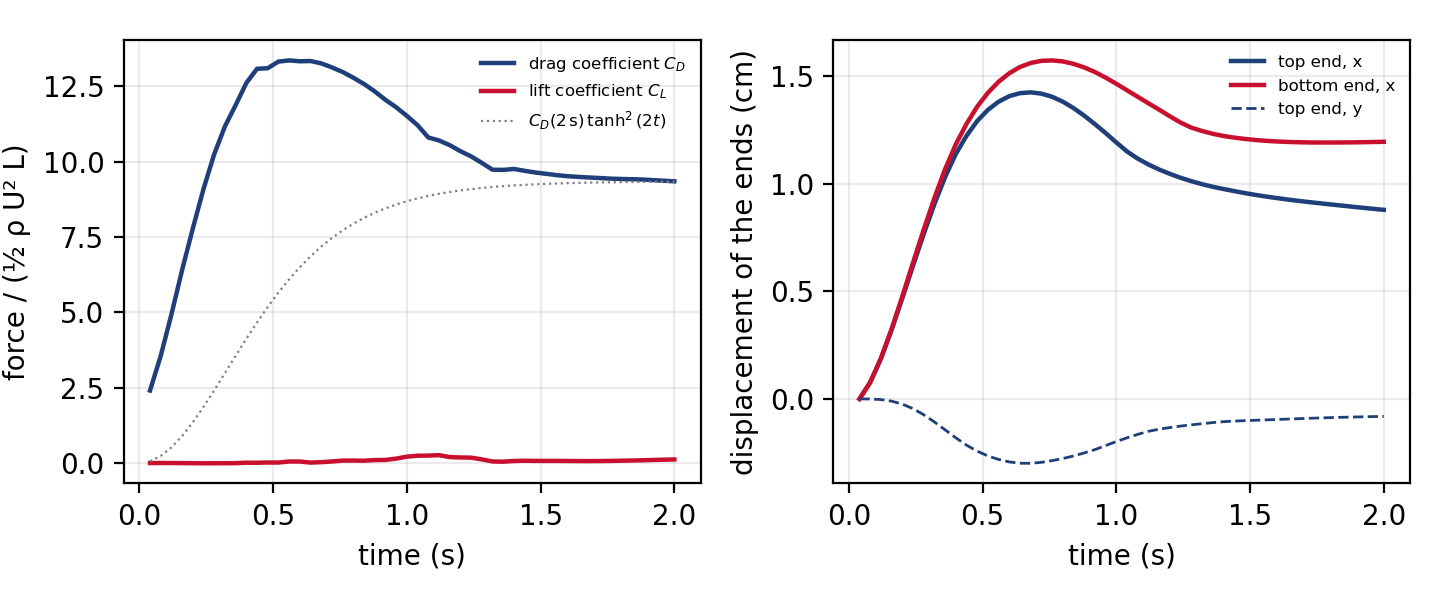
\includegraphics[width=\textwidth]{ch11-leaf-forces}
\end{column}
\begin{column}{0.42\textwidth}
\scriptsize Left: $C_D$ and $C_L$ against time; the dotted curve is $C_D(2\,\mathrm{s})\tanh^2(2t)$, what a force proportional to $U(t)^2$ would do. Right: the displacement of the leaf's two ends.
\vspace{1mm}

\scriptsize Measured (both scripts agree to the printed digits): $C_D$ rises with the ramp to $13.1$ at $t = 0.48$ s, where the stream has reached $75\%$ of its speed and the leaf is still bending, and decays to $9.3$ at $2$ s (mean $9.8$ over the second half); $C_L$ stays within $\pm 0.2$. The ends move $1.3$ cm downstream at $0.48$ s and settle at $0.9$ cm. In the 2013 convention ($F/(\rho U^2 L)$, half of these) the force at $2$ s is $4.7$.
\vspace{1mm}

\scriptsize The 2013 lecture's figure for this leaf (``Dimensionless force vs.\ time, $\mathrm{Re} = 2.5$'', over 20 s, from an impulsive start) showed the drag spiking to 7 in the first half second, ringing, and decaying to a plateau of $1.6$ by $t = 8$ s, with the lift at zero. The ramped start of this series' IB/03 removes the spike and the ringing; the decay is the same, and the plateau is reached only after several seconds, which the homework runs.
\end{column}
\end{columns}
\sourcecredit{IB/03 as shipped, IBAMR 0.19.0, 3 processes; \code{examples/analysis/leaf\_forces.py} (the MATLAB version gives the same table).}
\end{frame}

% 20
\begin{frame}{Positions: kinematics from the \code{X} files}
\label{fr:positions}
\small Everything measured in chapters 7--10 came from the \code{X} files with the reader of slide \ref{fr:pyreader}:
\begin{itemize}
  \item \al{a point}: the leaf's ends (chapter 7), the beam's tip (chapter 10): \code{X[k][i]} at time \code{t[k]};
  \item \al{an extent}: the band's diameter (chapter 8a), the plates' gap (chapter 9a), the tube's smallest opening (chapter 9b: the minimum over $i$ of $y_{\mathrm{top},i} - y_{\mathrm{bottom},i}$);
  \item \al{a cloud}: the pump's 121 markers, whose mean $x$ measured the net transport (chapter 9b), the fruit-fly plate's centroid and angle;
  \item \al{a shape against its target}: the curling beam's distance from its arc, the bell's width (chapter 10);
  \item \al{a velocity}: differences of positions over the dump interval, $(\mathbf{X}_i(t_{k+1}) - \mathbf{X}_i(t_k))/(t_{k+1} - t_k)$: crude but often enough; IBAMR's own \code{U} data could be written the same way as \code{X} (\code{getLData("U", ...)}) if you need it per step.
\end{itemize}
\vspace{1mm}
\footnotesize The 2013 MATLAB lecture's \code{positionread.m} and \code{readpositions.m} did this for one time (``returns vectors holding the $x$ and $y$ coordinates of the boundary points at one instance in time''), and \code{pcolor\_frames.m} overlaid the bell's points on the vorticity at ten times, ``really specific to jellyfish swimming: the $y$-position of the top of the bell is read, and all $y$-values are shifted. The top of the bell is always at position $y = 0$.'' That shift, subtracting a point's position from the others', is how a swimmer's shape is compared from pulse to pulse.
\end{frame}

% 21
\begin{frame}[fragile]{Several structures in one file}
\label{fr:structures}
\begin{columns}[T,onlytextwidth]
\begin{column}{0.52\textwidth}
\begin{lstlisting}[style=pythontiny]
# IB/07: two plates of 103 points, in the order of structure_names
t, F = read_series("hier_data_IB2d", "F", dt)
left, right = F[k][:103], F[k][103:]             # the index ranges of chapter 9a
print(left.sum(axis=0), right.sum(axis=0))       # equal and opposite pulls

# IB/11: the driving piece first, then tube (860), pericardium (1066), racetrack (3436), markers (121)
nd = 82                                          # actuator_top + actuator_bot in mode TARGET_VP
i_tube = nd
i_mark = nd + 860 + 1066 + 3436
tube = X[k][i_tube:i_tube + 860]
markers = X[k][i_mark:i_mark + 121]
work = sum((F[k][:nd] * (X[k + 1][:nd] - X[k][:nd])).sum() for k in range(len(t) - 1))   # the pump's W
\end{lstlisting}
\end{column}
\begin{column}{0.46\textwidth}
\scriptsize The files hold every structure, one after another, in the order of \code{structure\_names}; the point counts are the first lines of the \code{.vertex} files. So:
\begin{itemize}
  \item the sum over \emph{all} points mixes the forces on every structure: in IB/07 the two plates' pulls cancel, and the log's small \code{integral\{F\}} hides two forces of $63{,}000$ N (chapter 9a's README);
  \item sum over a structure's slice to get its force; sum over a sub-range for a part of it (the driven piece of the pump);
  \item the work a driven piece does, $W = \sum_{\mathrm{steps}}\sum_i \mathbf{F}_i\cdot\Delta\mathbf{X}_i$, needs both files at consecutive dumps and the dump interval small enough that $\Delta\mathbf{X}$ follows the motion: chapter 9b's pump coefficient;
  \item if \code{structure\_names} changes between runs (IB/11's five input files), the slices move: read the counts from the \code{.vertex} files rather than hard-coding them.
\end{itemize}
\end{column}
\end{columns}
\end{frame}

% 22
\begin{frame}[fragile]{Filtering}
\label{fr:filter}
\begin{columns}[T,onlytextwidth]
\begin{column}{0.5\textwidth}
\footnotesize ``Just like real data, immersed boundary points have noise due to vibrations. This is a smoothing function; control it with \code{windowSize}.'' (the lab's 2014 3D script)
\begin{lstlisting}[style=matlabtiny]
% the course (2012): a 9-point moving average, Curve Fitting Toolbox
force_smooth(:,1)=smooth(force(:,1),9);
% the lab (2014): a 90-point moving average with filter(), no toolbox; it lags by 45 samples
windowSize = 90;
force(:,1)=filter(ones(1,windowSize)/windowSize, 1, force(:,1));
\end{lstlisting}
\begin{lstlisting}[style=pythontiny]
# Python: a centred moving average of w samples (NumPy only)
w = 9
kernel = np.ones(w) / w
CD_smooth = np.convolve(CD, kernel, mode="same")   # the ends are biased; drop w//2 samples there
\end{lstlisting}
\end{column}
\begin{column}{0.48\textwidth}
\scriptsize Where the ripple comes from, and what to do:
\begin{itemize}
  \item the IB force on a point is a spring or tether force, and the points jitter by a fraction of a grid cell as they are advected across cells; the delta function makes the spread force depend on where in a cell a point sits. The ripple has the period of a point crossing a cell, $\Delta x/U$, and grows with stiffness;
  \item it is noise in the sense that it is not in the continuum problem; it averages to nothing over a few samples, and a moving average of 5--20 samples removes it. Make the dump interval short enough that the ripple is sampled (``more frequent than visit outputs for filtering'');
  \item \code{filter()} is one-sided and shifts the signal by half the window; \code{smooth()} and \code{np.convolve(..., 'same')} are centred;
  \item do not filter away the physics: a wingbeat sampled 20 times per period with a 9-point window loses its peaks. Plot raw and filtered together, as the course's figure did.
\end{itemize}
\end{column}
\end{columns}
\end{frame}

% 23
\begin{frame}[fragile]{In 3D: three numbers per point, and the lab's script}
\label{fr:threed}
\begin{columns}[T,onlytextwidth]
\begin{column}{0.54\textwidth}
\begin{lstlisting}[style=matlabtiny]
% a 2014 lab script for hier_data_IB3d (the header notes, shortened):
% If the script fails to run, the following are likely causes of failure:
% 1. If n=1 and fileID=-1, then the script was unable to open the first file:
%   a. Check the path_name ... don't end your pathname with a '/' ...
%   b. Check the starting_time ... you MUST have an F.10000 file in your data folder.
%   c. Check that the starting_time is 10,000 or greater. The data files for
%      time steps less than 10,000 have a leading zero (i.e. F.01000), which
%      MATLAB does not automatically write out.
% 2. If only some data is written out: check that the time_step from input2d is correct.
% 3. If your data isn't what you expected: double check length, velocity, density.
while ~(fileID==-1)
    fileID = fopen([path_name{1} '/hier_data_IB3d/F.' num2str(k)]);
    if (fileID==-1), break, end            % the end of the folder
    C=textscan(fileID,'%f','HeaderLines',3,'delimiter',' ','commentstyle','P');
    A=C{1}; fclose(fileID);
    force(n,1)=-2*sum(A(1:3:end))/(density*velocity^2*length);   % x
    force(n,2)=-2*sum(A(2:3:end))/(density*velocity^2*length);   % y
    force(n,3)=-2*sum(A(3:3:end))/(density*velocity^2*length);   % z
    n=n+1; k=k+time_step;
end
\end{lstlisting}
\end{column}
\begin{column}{0.44\textwidth}
\footnotesize
\begin{itemize}
  \item In 3D the folder is \code{hier\_data\_IB3d} and every point has $x$, $y$, $z$ in turn: \code{A(1:3:end)}, \code{A(2:3:end)}, \code{A(3:3:end)}; the readers of this series take \code{ndim = 3}.
  \item The script's normalization divides by $\rho U^2 L$ with $L$ a length: in 3D the coefficient wants an area $S$ (chapter 8b, $F/(\rho U^2 L^2)$); the script's ``force'' is then $C\cdot L$, fine for comparing runs of one geometry, wrong for comparing with a published $C_D$.
  \item The while loop stops at the first missing file, so a run that is still writing is read as far as it got.
  \item Its debugging notes are the three mistakes everyone makes: the path, the first file's number, the leading zeros. The series' readers list the folder instead of counting.
\end{itemize}
\end{column}
\end{columns}
\end{frame}

% 24
\begin{frame}{The 2013 MATLAB lecture: Eulerian data too}
\label{fr:tytell}
\small From \emph{Converting IBAMR output to MATLAB and analyzing it} (April 2013, and the 2020 Lecture 5):
\begin{itemize}
  \item ``Eric Tytell has Matlab code that reads data in the \code{visit\_dumps}, interpolates it, and outputs Matlab structures. When you open the folder, you need to run \code{install\_here.m}. The relevant Matlab files are in the CFD folder. I have added some additional files for reading and analyzing \code{hier\_data\_2d}.''
  \item ``It is necessary to not output Div U when running IBAMR due to the space in the name: \code{OUTPUT\_DIV\_U = FALSE}.''
  \item ``\code{[x,y,Vinterp,V] = importsamrai(pathname,'interpolaten',[GridSizex GridSizey])}: imports samrai data from files in the directory pathname. Files should be named \code{summary.samrai} and \code{processor\_clusterXXXXX.samrai}. \code{V} is the original visit data, and \code{Vinterp} is the interpolated data. The output \code{V} is a structure containing one element for each grid region: \code{V.level\_number}, \code{V.xlo}, \code{V.xup}, \code{V.rows}, \code{V.cols}, \code{V.U\_0}, \code{V.U\_1}, \code{V.P}, \code{V.F0}, \code{V.F1}, \code{V.Omega}.''
\end{itemize}
\end{frame}

% 24b
\begin{frame}{The 2013 MATLAB lecture: its functions}
\label{fr:tytell2}
\footnotesize
\begin{itemize}
  \item \code{Forceread.m}: ``takes the path name and the number of time steps and returns vectors holding the forces in the $x$ and $y$ directions at each of the boundary points for one instance in time.'' \code{positionread.m}: the same for the positions. (\code{readpositions.m} on a later slide is the same function under its other name.)
  \item \code{Force\_vs\_time.m}: ``will read in the force data from \code{hier\_data\_IB2d} and will determine the average dimensionless drag force acting on the structure vs.\ time. The force on each boundary point is summed. The high Re approximation that $F = C\rho S U^2$ is used to rescale the force.'' (The leaf figure of slide \ref{fr:leaf2}'s caption came from it.)
  \item \code{pcolor\_frames.m}: ``reads in positions from \code{hier\_data} and vorticities from \code{viz\_IB2d} samrai data and makes a $5\times2$ plot of vorticity at 10 times. This function is really specific to jellyfish swimming.''
  \item 2020: \code{flappy\_ends.m} (``imports SAMRAI data into Matlab, interpolates to a uniform grid, reads in the Lagrangian positions, and calculates the volumetric flow rate and maximum velocity at the end of the tube'') and \code{vol\_flow\_rate.m}, with the run's grid size, domain bounds, dump interval and point counts set by hand at the top of the script (\code{GridSizex = 4096}, \code{time\_step = 5000}, \code{timestep = 7.5e-6}, \code{pperitop = 5080}): the pattern of slide \ref{fr:dataread2}, with the same \code{timestep}/\code{time\_step} pair.
\end{itemize}
\vspace{1mm}
\footnotesize The Lagrangian half of that lecture is this chapter; the Eulerian half (SAMRAI files into MATLAB, interpolation to a uniform grid, flow rates across a line) is chapter 33, where the \code{importsamrai} tools are re-examined against VisIt's own export, which has become the simpler route.
\end{frame}

% 25
\begin{frame}{Other ways IBAMR gives you forces and positions}
\label{fr:other}
\small
\begin{itemize}
  \item \al{The Silo Lagrangian output} (\code{LSiloDataWriter}, registered in every example's \code{main.cpp}): \code{viz\_IB2d/lag\_data.visit}, the structures as meshes for VisIt (chapter 26). Positions only, at the visualization interval; VisIt can export them, but the \code{X} files are the direct route.
  \item \al{The upstream examples' own post-processing}: \code{examples/IB/explicit/ex2} (a cylinder) computes its drag and lift inside the program each step and writes them to a text file; the IBFE examples \code{ex5}, \code{ex6}, \code{ex11} do the same with the finite-element force (Part IV). The pattern is a function called after \code{advanceHierarchy} that sums the forces it wants and appends a line: a lighter alternative to dumping every point when only the totals are needed.
  \item \al{Callbacks}: the integrator accepts functions to run before or after each step (chapter 9b used the pre-step hook for the pump); a post-step callback can sum forces or sample positions without touching the main loop.
  \item \al{Restart files} hold everything but are not for analysis.
  \item \al{IBFE} (Part IV) has its own force and position output through libMesh's ExodusII files and VisIt; chapter 20's examples show it.
\end{itemize}
\end{frame}

% 26
\begin{frame}{Energies and work from $\mathbf{F}$ and $\mathbf{X}$}
\label{fr:energy}
\small With both files at every dump you can compute the quantities the chapters before asked for:
\begin{itemize}
  \item \al{work done by a driven structure} (chapter 9b's pump coefficient): $W = \sum_{\mathrm{dumps}}\sum_{i \in \mathrm{driven}} \mathbf{F}_i\cdot\big(\mathbf{X}_i(t_{k+1}) - \mathbf{X}_i(t_k)\big)$; the dump interval must resolve the motion, and the sign tells whether the structure pushes the fluid or is pushed;
  \item \al{stretching and bending energy} (chapter 10's homework): $E_s = \sum \frac12 K_{\mathrm{file}}(R - R_0)^2$ over the springs and $E_b = \sum \frac12 K_{\mathrm{file}}|\mathbf{X}_{i-1} - 2\mathbf{X}_i + \mathbf{X}_{i+1} - \mathbf{C}_i|^2$ over the beams, from the positions and the stiffnesses in the structure files (the file stiffnesses already carry the $\Delta s$ factors, so these are energies per unit depth);
  \item \al{power into the fluid}: $P = \sum_i \mathbf{F}_i\cdot\mathbf{U}_i$, with $\mathbf{U}_i$ from differences of positions or from \code{getLData("U", ...)};
  \item \al{a force balance check}: the sum over a tethered structure equals minus the fluid force; over a free structure it is zero; over everything in a periodic box it is the net force on the fluid, which must be balanced by a mean pressure gradient (chapter 7's note on periodic domains).
\end{itemize}
\vspace{1mm}
\begin{punchbox}
\footnotesize Chapter 8b's dimensionless outputs ($F'$, $C_{\mathrm{pump}}$, Strouhal numbers) are all one of these divided by $\rho$, $U$ and $L$. Compute them from the files, not by eye from VisIt.
\end{punchbox}
\end{frame}

% 27
\begin{frame}{What can go wrong}
\label{fr:wrong}
\scriptsize
\begin{tabular}{@{}L{0.3\textwidth}L{0.62\textwidth}@{}}
\toprule
The mistake & What happens\\
\midrule
the sign & a drag that is negative: the file holds the force on the fluid; the force on the body is minus the sum\\
the $\frac12$ & coefficients twice too large or small, and the 2013 ``divide by 2'' myth. Say which convention you use\\
three header lines assumed & a file from one process may have fewer: the first $x$ is lost and every point's $x$ and $y$ swap. Keep lines that are numbers\\
\code{num2str(k)} for the file name & no file below step 10,000 is found (\code{F.01000}); list the folder instead\\
files sorted as strings & \code{X.10000} before \code{X.00800} if leading zeros are missing; sort by the step number\\
all structures summed & the plates' pulls cancel, the pump's tube hides the actuator; slice by \code{structure\_names}\\
\code{timestep} and \code{time\_step} & the step size and the dump interval, confused in a dozen lab scripts; name them \code{dt} and \code{interval}\\
too coarse a dump & a wingbeat sampled 4 times per period looks like noise; no filter helps\\
too wide a filter & the peaks of a periodic force are flattened and shifted; plot raw and filtered\\
a loose Stokes tolerance & a force ripple that is not vibration; \code{-stokes\_ksp\_rtol 1e-12} (chapter 16) to test\\
3D force divided by a length & a coefficient times a length; use an area\\
\bottomrule
\end{tabular}
\end{frame}

% 28
\begin{frame}{Homework}
\label{fr:hw}
\begin{columns}[T,onlytextwidth]
\begin{column}{0.56\textwidth}
\footnotesize From the 2012--2020 courses and this chapter (Appendix C collects the full set):
\begin{enumerate}
  \item IB/03: run the course's 20 s (\code{END\_TIME = 20.0}) and plot $C_D$ to the plateau; compare with the 2013 figure's $1.6$. Then halve $\mu$ and say what happens to the plateau and to the ripple.
  \item IB/07: the force on each plate against time from the \code{F} files (chapter 9a's README table), with the gap from the \code{X} files on the same axes.
  \item IB/11: the work done by the actuator over the second period and the pump coefficient (chapter 9b), for the target-point and the applied-force modes.
  \item IB/10: the bell's vertical force (the sum over the bell, which should be zero) and the apex's velocity from differences of positions; is the jellyfish accelerating during contraction or expansion?
  \item Write the energy of IB/09's beam from the \code{X} files and the stiffnesses, and plot it against time.
\end{enumerate}
\end{column}
\begin{column}{0.43\textwidth}
\begin{punchbox}
\scriptsize What to hand in: the reader you used, the normalization (with $\rho$, $U$, $L$ and the convention), the raw and the filtered curve on one plot, and one sentence on the sign of each force.
\end{punchbox}
\scriptsize Extension: rerun IB/03 with \code{-stokes\_ksp\_rtol 1e-12} and overlay the two raw $C_D$ curves.
\end{column}
\end{columns}
\end{frame}

% 29
\begin{frame}{Rules of thumb}
\label{fr:thumb}
\small
\begin{itemize}
  \item The file holds forces on points, on the fluid. Sum a structure's slice; negate for the force on the body.
  \item Keep lines that are numbers; sort by step number; the time is step $\times$ \code{DT}.
  \item $x, y[, z]$ alternate per point; in Python \code{[:, 0]}, \code{[:, 1]}; in MATLAB \code{(:, 1)}, \code{(:, 2)}.
  \item One normalization, stated: $C = F/(\frac12\rho U^2 S)$ or $F' = F/(\rho U^2 L)$.
  \item Reproduce the log's \code{integral\{F\}} before trusting anything else.
  \item Dump often enough to see the ripple, filter it with a centred window, show both.
  \item Positions give kinematics; positions and forces together give work and energy.
  \item Structures sit in the file in input order; slice, never sum blindly.
\end{itemize}
\end{frame}

% 30
\begin{frame}{Summary}
\label{fr:summary}
\footnotesize
\begin{enumerate}
  \item IBAMR's Lagrangian force is a force on each point, not a density, and the $\Delta s$ in every stiffness is that conversion. The examples write it, with the positions, as PETSc ASCII vectors every \code{data\_dump\_interval} steps, in Lagrangian order, from their own \code{output\_data()}.
  \item The sum over a structure is its tether and applied force, minus the fluid's force on it; a free body sums to zero. The course's coefficient divides by $\frac12\rho U^2 S$, chapter 8b's by $\rho U^2 L$; the ``divide by 2'' of 2013 was that $\frac12$.
  \item The readers of this series keep every numeric line, sort by step and return one row per point, in Python and in MATLAB; \code{leaf\_forces} shows the whole analysis on IB/03 in a dozen lines, with the same numbers from both.
  \item Positions give every kinematic quantity the earlier chapters measured; positions and forces give work and energy; several structures are slices of the same file.
  \item Filter the cell-crossing ripple with a centred moving average and show the raw signal too; tighten the Stokes tolerance to tell ripple from solver noise.
\end{enumerate}
\begin{homebox}
\footnotesize Next, chapter 12: 3D simulations, where the files have three numbers per point and the structures are sheets and bristles.
\end{homebox}
\end{frame}

% 31
\begin{frame}{What changed since the older course notes}
\label{fr:changed}
\footnotesize
\begin{itemize}
  \item The file format is shown from a current file and the writer is quoted; the ``three header lines'' of the course scripts is explained and replaced by readers that do not count them, in both languages, shipped in \code{examples/analysis} and tested.
  \item The 2013 ``scaling error, divide by 2'' is retired with its explanation; the sign and the $\frac12$ are stated once.
  \item The fruit-fly example, no longer available, is described from its slides and figure (the figure itself, with a personal path in its title, is not reproduced); the method is demonstrated on IB/03 with a measured table and a comparison to the 2013 leaf figure.
  \item The lab's 2014 3D script is quoted for its debugging notes and its 3D indexing, with its author's personal path removed; its normalization by a length is flagged.
  \item New: what the sum of the forces means structure by structure, slicing several structures, work and energy from the two files, the origin of the ripple and how to filter it, the Stokes tolerance, and the other outputs IBAMR has.
  \item The Eulerian half of the 2013 MATLAB lecture is moved to chapter 33.
\end{itemize}
\end{frame}

% 33
\begin{frame}{References}
\label{fr:refs}
\scriptsize
\begin{itemize}
  \item IBAMR: \code{examples/IB/explicit/ex1/example.cpp} (\code{output\_data}, the origin of the examples' writer, with the HDF5 Eulerian output), \code{examples/IB/explicit/ex2} (drag and lift in the program); \code{include/ibtk/LDataManager.h} (\code{getLData}, \code{scatterPETScToLagrangian}), \code{LSiloDataWriter.h}. \url{https://github.com/IBAMR/IBAMR}; the FAQ, \url{https://github.com/IBAMR/IBAMR/wiki/FAQ}.
  \item PETSc: \code{VecView} and the ASCII viewer, \url{https://petsc.org/release/manualpages/Vec/VecView/}.
  \item This series: \code{examples/analysis/} (\code{hier\_data.py}, \code{read\_hier\_data.m}, \code{read\_input.m}, \code{leaf\_forces.py}, \code{leaf\_forces.m}); the \code{tools/ch*\_figures.py} scripts of chapters 7--10; chapter 8b (dimensionless forces), chapter 9b (the pump coefficient), chapter 33 (Eulerian data into MATLAB).
  \item The public course folder \code{Reading-Forces}: \code{dataread2.m} (2012--2013) and the lab's 2014 3D script.
  \item Sources: \emph{IBAMR Forces} (MATH 769, February 26, 2012, 8 slides) and its editions \emph{IBAMR Tutorial: Output and Analyze Forces} (public folder 7, 2017) and \emph{Lecture 15: Output and Analyze Forces} (2015); \emph{Converting IBAMR output to Matlab and analyzing it} (MATH 769, April 23, 2013, 12 slides); \emph{5: Reading forces and converting IBAMR output to Matlab and analyzing it} (2020, 24 slides).
\end{itemize}
\end{frame}

\end{document}
